% =====================================================================
%  Capítulo 30 - Polinômios e a FFT
%  PPGEC2316 - Algoritmos de Engenharia (UFRN)
%  Referência: Cormen, Leiserson, Rivest, Stein.
%              Introduction to Algorithms, 4th ed., MIT Press, 2022 (Cap. 30).
%  Compilar com pdflatex (2x), xelatex ou no Overleaf.
% =====================================================================
\documentclass[aspectratio=169,10pt]{beamer}

\usetheme[progressbar=frametitle,numbering=fraction,block=fill,sectionpage=none]{metropolis}

\usepackage{babel}
\babelprovide[import,main]{portuguese}
\usepackage{iftex}
\ifPDFTeX
  \usepackage[utf8]{inputenc}
  \usepackage[T1]{fontenc}
\fi
\usepackage{amsmath,amssymb,bm}
\usepackage{booktabs}
\usepackage{tikz}
\usetikzlibrary{arrows.meta,positioning,calc,fit,backgrounds,
  decorations.pathreplacing,babel}

% ---------------------------------------------------------------------
% Cores (mesmas da apresentação DCNN)
% ---------------------------------------------------------------------
\definecolor{verde}{HTML}{1E6B2E}
\definecolor{verdeclaro}{HTML}{E8F3EA}
\definecolor{laranja}{HTML}{C0561B}
\definecolor{laranjaclaro}{HTML}{FBEDE4}
\definecolor{azul}{HTML}{1F4E79}
\definecolor{azulclaro}{HTML}{E6EEF6}
\setbeamercolor{block title}{bg=verde,fg=white}
\setbeamercolor{block body}{bg=verdeclaro,fg=black}
\setbeamercolor{block title alerted}{bg=laranja,fg=white}
\setbeamercolor{block body alerted}{bg=laranjaclaro,fg=black}
\setbeamercolor{block title example}{bg=azul,fg=white}
\setbeamercolor{block body example}{bg=azulclaro,fg=black}
\setbeamercolor{alerted text}{fg=black}

% Roteiro no início de cada seção (como no Cap. 10)
\AtBeginSection[]{%
  \begin{frame}{Roteiro}
    \tableofcontents[currentsection]
  \end{frame}}

% ---------------------------------------------------------------------
% Pseudocódigo no estilo do livro (CLRS, 4a ed.)
% ---------------------------------------------------------------------
\newcounter{pcline}
\newlength{\pcind}\setlength{\pcind}{1.2em}
% \begin{pseudo}[tamanho]{cabeçalho} ... \end{pseudo}
\newenvironment{pseudo}[2][\footnotesize]{%
  \par\noindent\begin{minipage}{\linewidth}#1\normalfont\rmfamily
  \setlength{\parindent}{0pt}\setlength{\parskip}{0pt}%
  \setcounter{pcline}{0}%
  #2\par\smallskip}%
  {\par\end{minipage}\par}
% \li[nível de indentação] linha numerada
\newcommand{\li}[1][0]{\par\stepcounter{pcline}%
  \hangindent=\dimexpr2.6em+#1\pcind+\pcind\relax\hangafter=1
  \makebox[1.2em][r]{\tiny\color{gray}\arabic{pcline}}\hspace{0.8em}%
  \hspace*{#1\pcind}\ignorespaces}
\newcommand{\Cm}[1]{\hfill{\color{gray!70!black}\ // #1}}
\newcommand{\kw}[1]{\textbf{#1}}
\newcommand{\IF}{\kw{if}\ }
\newcommand{\FOR}{\kw{for}\ }
\newcommand{\TO}{\ \kw{to}\ }
\newcommand{\DOWNTO}{\ \kw{downto}\ }
\newcommand{\RETURN}{\kw{return}\ }
\newcommand{\proc}[1]{\textnormal{\rmfamily\textsc{#1}}}
\newcommand{\eqq}{\mathrel{=\!=}}

% ---------------------------------------------------------------------
% Notação
% ---------------------------------------------------------------------
\newcommand{\w}[2][n]{\omega_{#1}^{#2}}       % \w{k} = omega_n^k
\newcommand{\Aev}{A^{\mathrm{even}}}
\newcommand{\Aod}{A^{\mathrm{odd}}}
\newcommand{\yev}{y^{\mathrm{even}}}
\newcommand{\yod}{y^{\mathrm{odd}}}
\newcommand{\DFT}{\mathrm{DFT}}

% ---------------------------------------------------------------------
% Estilos TikZ
% ---------------------------------------------------------------------
\tikzset{
  >={Stealth[length=2mm]},
  bloco/.style={draw=black, line width=0.8pt, rounded corners=3pt,
    minimum width=2.6cm, minimum height=0.9cm, align=center,
    font=\footnotesize, fill=white},
  destaque/.style={bloco, fill=verdeclaro, draw=verde},
  seta/.style={-{Stealth[length=6pt]}, line width=1.4pt, draw=gray!70!black},
  raiz/.style={circle, fill=verde, inner sep=0pt, minimum size=5pt},
  tnode/.style={draw, rounded corners=2pt, fill=white, font=\scriptsize,
    inner sep=2pt, align=center},
  fio/.style={draw=gray!70, thick},
  bf/.style={draw=verde, line width=1.4pt},
  bfdot/.style={circle, fill=verde, inner sep=0pt, minimum size=4pt},
}

% ---------------------------------------------------------------------
\title{Capítulo 30 -- Polinômios e a FFT}
\subtitle{PPGEC2316 -- Algoritmos de Engenharia}
\author{Raphael Ramos \\ Leandro de Souza \\ Julia Alanne}
\institute{Universidade Federal do Rio Grande do Norte -- UFRN}
\date{}

\begin{document}

\maketitle

\begin{frame}{Roteiro}
  \tableofcontents
\end{frame}

% =====================================================================
\section{Introdução}
% =====================================================================

\begin{frame}{Motivação}
  \begin{itemize}
    \item Somar dois polinômios de grau $n$: $\Theta(n)$.
    \item Multiplicá-los pelo método ``escolar'': $\Theta(n^2)$.
    \item A \textbf{transformada rápida de Fourier} (FFT) reduz a multiplicação
          para $\Theta(n\lg n)$.
    \item Aplicação mais comum: Processamento de Sinais
      \begin{itemize}
        \item domínio do tempo $\leftrightarrow$ domínio da frequência;
        \item compressão de áudio e vídeo (ex.: MP3), filtros, imagens.
      \end{itemize}
  \end{itemize}
  \vspace{4pt}
  \begin{block}{Pergunta central}
    Como multiplicar dois polinômios de grau $n$ em menos que
    $\Theta(n^2)$?
  \end{block}
  \vspace{4pt}
  {\small Neste capítulo, $i$ denota exclusivamente $\sqrt{-1}$.}
\end{frame}

\begin{frame}{Polinômios}
  \begin{block}{Definição (polinômio)}
    Um polinômio na variável $x$ sobre um corpo $F$ (tipicamente $\mathbb{C}$) é
    \[
      A(x) = \sum_{j=0}^{n-1} a_j x^j,
    \]
    com \textbf{coeficientes} $a_0,a_1,\dots,a_{n-1}$.
    \begin{itemize}
      \item \textbf{Grau}: $k$, se $a_k$ é o coeficiente não nulo de maior índice.
      \item \textbf{Limite de grau} (\textit{degree-bound}): qualquer inteiro
            \alert{estritamente maior} que o grau.
    \end{itemize}
  \end{block}
  \begin{exampleblock}{Exemplo}
    $A(x) = 6x^3 + 7x^2 - 10x + 9$ \;$\Rightarrow$\; grau $3$; \;
    limites de grau válidos: $4, 5, 6, \dots$\\
    Com limite de grau $n=4$: vetor de coeficientes $(a_0,a_1,a_2,a_3) = (9,-10,7,6)$.
  \end{exampleblock}
\end{frame}

\begin{frame}{Soma e multiplicação}
  \begin{columns}[T]
    \begin{column}{0.48\textwidth}
      \textbf{Soma} ($\Theta(n)$): $c_j = a_j + b_j$.\\[3pt]
      {\small $(6x^3+7x^2-10x+9) + (-2x^3+4x-5)$\\
      $= 4x^3+7x^2-6x+4$}

      \vspace{8pt}
      \textbf{Multiplicação}: se $A$ e $B$ têm limite de grau $n$, então
      $C=AB$ tem limite de grau $2n-1$ e
      \[
        c_j = \sum_{k=0}^{j} a_k\, b_{j-k}.
      \]
      O vetor $c$ é a \textbf{convolução} $c = a \otimes b$.\\
      Cada $a_k$ multiplica cada $b_l$: \alert{$\Theta(n^2)$}.
    \end{column}
    \begin{column}{0.48\textwidth}
      \begin{exampleblock}{Exemplo (convolução)}
        $A(x) = 1 + 2x$, \; $B(x) = 3 + x$ \;\; ($a=(1,2)$, $b=(3,1)$)
        \begin{align*}
          c_0 &= a_0b_0 = 1\cdot 3 = 3\\
          c_1 &= a_0b_1 + a_1b_0 = 1\cdot1 + 2\cdot3 = 7\\
          c_2 &= a_1b_1 = 2\cdot1 = 2
        \end{align*}
        $\Rightarrow\; C(x) = 3 + 7x + 2x^2$.
      \end{exampleblock}
    \end{column}
  \end{columns}
\end{frame}

% =====================================================================
\section{Representação de polinômios}
% =====================================================================

\begin{frame}{Representação por coeficientes}
  \begin{block}{Definição}
    Um polinômio de limite de grau $n$ é representado pelo vetor
    $a = (a_0, a_1, \dots, a_{n-1})$.
  \end{block}
  \vspace{6pt}
  Na representação por coeficientes:
  \begin{itemize}
    \item soma de dois polinômios: $\Theta(n)$;
    \item multiplicação de dois polinômios: $\Theta(n^2)$.
    \item avaliação em um ponto $x_0$: $\Theta(n)$ (Regra de Horner);
  \end{itemize}
\end{frame}

\begin{frame}{Regra de Horner}
  \begin{columns}[T]
    \begin{column}{0.5\textwidth}
      A avaliação de um polinômio em $x = x_0$ pode ser feita começando
      do último coeficiente ($a_{n-1}$).\\[4pt]
      \textbf{Avaliar} $A(x_0)$ com a \textbf{regra de Horner} em $\Theta(n)$:
      \[
        A(x_0) = a_0 + x_0\big(a_1 + x_0(a_2 + \cdots + x_0(a_{n-1}))\big)
      \]
      \begin{pseudo}[\small]{\proc{Horner}$(a, n, x_0)$}
        \li $y = a_{n-1}$
        \li \FOR $j = n-2$ \DOWNTO $0$
        \li[1] $y = a_j + x_0 \cdot y$
        \li \RETURN $y$
      \end{pseudo}
    \end{column}
    \begin{column}{0.46\textwidth}
      \begin{exampleblock}{Exemplo (Horner)}
        $A(x) = 1 + 2x + 3x^2$ em $x_0 = 2$:
        \begin{center}
          \begin{tabular}{ccc}
            \toprule
            $j$ & $a_j$ & $y$ \\
            \midrule
            -- & -- & $3$ \\
            $1$ & $2$ & $2 + 2\cdot 3 = 8$ \\
            $0$ & $1$ & $1 + 2\cdot 8 = 17$ \\
            \bottomrule
          \end{tabular}
        \end{center}
        Conferindo: $1 + 4 + 12 = 17$.
      \end{exampleblock}
    \end{column}
  \end{columns}
\end{frame}

\begin{frame}{Representação por pontos (\textit{point-value})}
  \begin{columns}[T]
    \begin{column}{0.52\textwidth}
      \begin{block}{Definição}
        Uma representação por pontos de $A$, de limite de grau $n$, é um conjunto de
        $n$ pares
        \[
          \{(x_0,y_0),(x_1,y_1),\dots,(x_{n-1},y_{n-1})\}
        \]
        com os $x_k$ \textbf{distintos} e $y_k = A(x_k)$.
      \end{block}
      \begin{itemize}
        \item \textbf{Avaliação}: coeficientes $\to$ pontos (Horner em $n$ pontos: $\Theta(n^2)$).
        \item \textbf{Interpolação}: pontos $\to$ coeficientes.
        \item Há infinitas representações por pontos: qualquer escolha de $n$ pontos distintos serve.
      \end{itemize}
    \end{column}
    \begin{column}{0.44\textwidth}
      \begin{exampleblock}{Exemplo}
        $A(x) = 1 + 2x + 3x^2$ ($n=3$), nos pontos $0, 1, -1$:
        \begin{align*}
          A(0)  &= 1\\
          A(1)  &= 1+2+3 = 6\\
          A(-1) &= 1-2+3 = 2
        \end{align*}
        Representação: $\{(0,1),(1,6),(-1,2)\}$.
      \end{exampleblock}
      \centering
      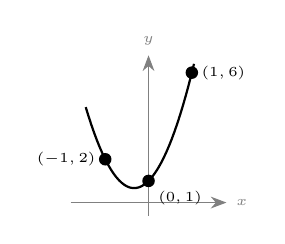
\begin{tikzpicture}[scale=0.55]
        \draw[->, gray] (-1.8,0) -- (1.8,0) node[right, font=\tiny] {$x$};
        \draw[->, gray] (0,-0.3) -- (0,3.4) node[above, font=\tiny] {$y$};
        \draw[black, thick, domain=-1.45:1.05, samples=40]
          plot (\x, {(1 + 2*\x + 3*\x*\x)/2});
        \foreach \p/\q in {0/1, 1/6, -1/2}
          \node[circle, fill=black, inner sep=1.6pt] at (\p, \q/2) {};
        \node[font=\tiny, right] at (1,3) {$(1,6)$};
        \node[font=\tiny, left]  at (-1,1) {$(-1,2)$};
        \node[font=\tiny, below right] at (0,0.5) {$(0,1)$};
      \end{tikzpicture}
    \end{column}
  \end{columns}
\end{frame}

\begin{frame}{Unicidade da interpolação}
  \begin{block}{Teorema 30.1 (unicidade do polinômio interpolador)}
    Para quaisquer $n$ pares $\{(x_k,y_k)\}$ com $x_k$ distintos, existe um
    \textbf{único} polinômio $A$ de limite de grau $n$ com $y_k = A(x_k)$,
    $k = 0,\dots,n-1$.
  \end{block}
  \begin{columns}[T]
    \begin{column}{0.5\textwidth}
      \small
      \textbf{Prova:} $y_k = A(x_k)$ equivale ao sistema
      \[
        \underbrace{\begin{pmatrix}
          1 & x_0 & \cdots & x_0^{n-1}\\
          1 & x_1 & \cdots & x_1^{n-1}\\
          \vdots & \vdots & \ddots & \vdots\\
          1 & x_{n-1} & \cdots & x_{n-1}^{n-1}
        \end{pmatrix}}_{V(x_0,\dots,x_{n-1})\ \text{(Vandermonde)}}
        \begin{pmatrix} a_0\\ a_1\\ \vdots\\ a_{n-1}\end{pmatrix}
        =
        \begin{pmatrix} y_0\\ y_1\\ \vdots\\ y_{n-1}\end{pmatrix}
      \]
      com $\det V = \prod_{j<k}(x_k - x_j) \neq 0$. Logo $a = V^{-1}y$.\\[3pt]
      Resolver o sistema: $O(n^3)$.
    \end{column}
    \begin{column}{0.46\textwidth}
      \begin{exampleblock}{Exemplo}
        Pontos $x = (0, 1, -1)$:
        \[
          V = \begin{pmatrix} 1&0&0\\ 1&1&1\\ 1&-1&1 \end{pmatrix}
        \]
        $\det V = (1-0)(-1-0)(-1-1) = 2 \neq 0$.\\
        Resolvendo $Va = (1,6,2)^T$:
        $a_0 = 1$, $a_1+a_2 = 5$, $-a_1+a_2 = 1$\\
        $\Rightarrow a = (1, 2, 3)$: $A(x) = 1 + 2x + 3x^2$.
      \end{exampleblock}
    \end{column}
  \end{columns}
\end{frame}

\begin{frame}{Interpolação de Lagrange}
  \begin{columns}[T]
    \begin{column}{0.46\textwidth}
      Algoritmo mais rápido ($\Theta(n^2)$), pela \textbf{fórmula de Lagrange}:
      \[
        A(x) = \sum_{k=0}^{n-1} y_k \,
        \frac{\prod_{j\neq k}(x - x_j)}{\prod_{j\neq k}(x_k - x_j)}
      \]
      \begin{itemize}
        \item Cada fração vale $1$ em $x_k$ e $0$ nos demais $x_j$.
        \item Avaliação e interpolação são \textbf{operações inversas} bem definidas.
      \end{itemize}
      \begin{alertblock}{Observação}
        \small Interpolação é numericamente delicada: pequenos erros de arredondamento
        podem gerar grandes diferenças no resultado.
      \end{alertblock}
    \end{column}
    \begin{column}{0.5\textwidth}
      \begin{exampleblock}{Exemplo}
        Pontos $\{(0,1),(1,6),(-1,2)\}$:
        \begin{align*}
          A(x) &= 1\cdot\frac{(x-1)(x+1)}{(0-1)(0+1)}
                 + 6\cdot\frac{x(x+1)}{(1)(2)}\\
               &\quad + 2\cdot\frac{x(x-1)}{(-1)(-2)}\\
               &= -(x^2-1) + 3(x^2+x) + (x^2-x)\\
               &= 3x^2 + 2x + 1. \
        \end{align*}
      \end{exampleblock}
    \end{column}
  \end{columns}
\end{frame}

\begin{frame}{Operações na representação por pontos}
  \begin{columns}[T]
    \begin{column}{0.5\textwidth}
      Se $A$ e $B$ são avaliados \textbf{nos mesmos pontos}:
      \begin{itemize}
        \item \textbf{Soma}: $C(x_k) = A(x_k) + B(x_k)$ \;\; $\Theta(n)$.
        \item \textbf{Produto}: $C(x_k) = A(x_k)\,B(x_k)$ \;\; $\Theta(n)$!
      \end{itemize}
      \begin{alertblock}{Cuidado}
        $C = AB$ tem limite de grau $2n$, então precisa de $2n$ pontos.
        Use representações \textbf{estendidas} de $A$ e $B$, com $2n$ pontos cada.
      \end{alertblock}
    \end{column}
    \begin{column}{0.46\textwidth}
      \begin{exampleblock}{Exemplo}
        $A(x) = 1 + x$, \; $B(x) = 2 + x$ ($n=2$). Pontos $x = 0,1,2,3$:
        \begin{center}
          \begin{tabular}{ccccc}
            \toprule
            $x_k$ & $0$ & $1$ & $2$ & $3$ \\
            \midrule
            $A(x_k)$ & $1$ & $2$ & $3$ & $4$ \\
            $B(x_k)$ & $2$ & $3$ & $4$ & $5$ \\
            $C(x_k)$ & $2$ & $6$ & $12$ & $20$ \\
            \bottomrule
          \end{tabular}
        \end{center}
        Interpolando: $C(x) = 2 + 3x + x^2$. Confere: $C(3) = 2+9+9 = 20$.\\[2pt]
        {\small Com só 2 pontos ($x=0,1$), infinitas parábolas passariam por $(0,2)$ e $(1,6)$.}
      \end{exampleblock}
    \end{column}
  \end{columns}
\end{frame}

\begin{frame}{Multiplicação rápida: a estratégia}
  \centering
  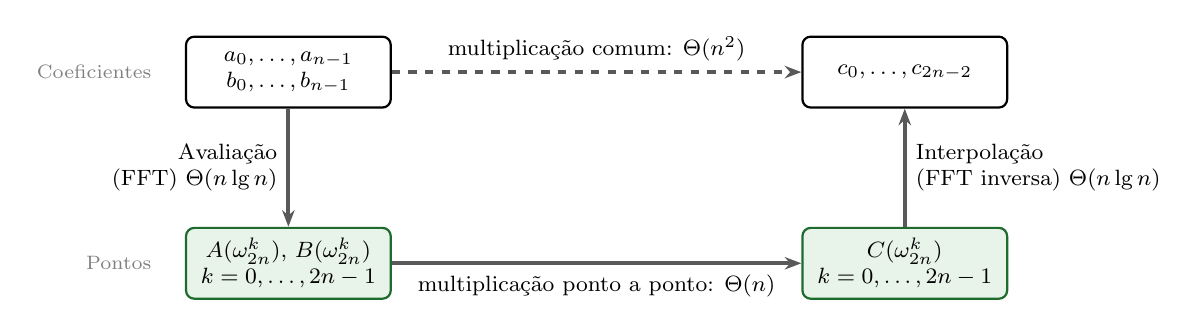
\begin{tikzpicture}[node distance=0.4cm]
    \node[bloco] (ab) {$a_0,\dots,a_{n-1}$\\ $b_0,\dots,b_{n-1}$};
    \node[bloco, right=5.2cm of ab] (c) {$c_0,\dots,c_{2n-2}$};
    \node[destaque, below=1.5cm of ab] (pv) {$A(\w[2n]{k}),\,B(\w[2n]{k})$\\ $k=0,\dots,2n-1$};
    \node[destaque, below=1.5cm of c] (cv) {$C(\w[2n]{k})$\\ $k=0,\dots,2n-1$};
    \draw[seta, dashed] (ab) -- node[above, font=\footnotesize] {multiplicação comum: $\Theta(n^2)$} (c);
    \draw[seta] (ab) -- node[left, font=\footnotesize, align=right] {Avaliação\\ (FFT) $\Theta(n\lg n)$} (pv);
    \draw[seta] (pv) -- node[below, font=\footnotesize] {multiplicação ponto a ponto: $\Theta(n)$} (cv);
    \draw[seta] (cv) -- node[right, font=\footnotesize, align=left] {Interpolação\\ (FFT inversa) $\Theta(n\lg n)$} (c);
    \node[left=0.3cm of ab, font=\scriptsize, align=right, text=gray] {Coeficientes};
    \node[left=0.3cm of pv, font=\scriptsize, align=right, text=gray] {Pontos};
  \end{tikzpicture}

  \vspace{6pt}
  \begin{columns}[T]
    \begin{column}{0.55\textwidth}
      \small
      \begin{enumerate}
        \item \textbf{Dobrar o limite de grau}: completar com $n$ zeros. \hfill $\Theta(n)$
        \item \textbf{Avaliar}: FFT de ordem $2n$ em $A$ e $B$. \hfill $\Theta(n\lg n)$
        \item \textbf{Multiplicar ponto a ponto}. \hfill $\Theta(n)$
        \item \textbf{Interpolar}: FFT inversa. \hfill $\Theta(n\lg n)$
      \end{enumerate}
    \end{column}
    \begin{column}{0.4\textwidth}
      \begin{block}{Teorema 30.2}
        \small Dois polinômios de limite de grau $n$, em coeficientes, podem ser
        multiplicados em $\Theta(n\lg n)$.
      \end{block}
    \end{column}
  \end{columns}
\end{frame}

% =====================================================================
\section{Raízes complexas da unidade}
% =====================================================================

\begin{frame}{Raízes complexas da unidade}
  \begin{columns}[T]
    \begin{column}{0.55\textwidth}
      \begin{block}{Definição}
        Uma \textbf{raiz complexa $n$-ésima da unidade} é um $\omega \in \mathbb{C}$ com
        $\omega^n = 1$. Existem exatamente $n$ delas:
        \[
          e^{2\pi i k/n},\quad k = 0,1,\dots,n-1,
        \]
        onde $e^{iu} = \cos u + i\sin u$.\\[2pt]
        \textbf{Raiz principal}: $\omega_n = e^{2\pi i/n}$; as demais são
        suas potências $\w{0},\w{1},\dots,\w{n-1}$.
      \end{block}
      \begin{exampleblock}{Exemplo ($n=4$)}
        $\omega_4 = e^{2\pi i/4} = \cos\frac{\pi}{2} + i\sin\frac{\pi}{2} = i$.\\
        Raízes: $\w[4]{0}=1,\ \w[4]{1}=i,\ \w[4]{2}=-1,\ \w[4]{3}=-i$.\\
        Conferindo: $i^4 = (i^2)^2 = (-1)^2 = 1$.
      \end{exampleblock}
    \end{column}
    \begin{column}{0.41\textwidth}
      \centering
      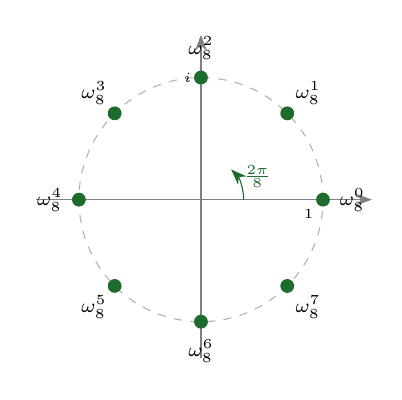
\begin{tikzpicture}[scale=1.55]
        \draw[->, gray] (-1.35,0) -- (1.4,0);
        \draw[->, gray] (0,-1.3) -- (0,1.35);
        \draw[gray!60, dashed] (0,0) circle (1);
        \foreach \k in {0,...,7} {
          \node[raiz] (r\k) at ({45*\k}:1) {};
          \node[font=\scriptsize] at ({45*\k}:1.24) {$\w[8]{\k}$};
        }
        \draw[verde, ->] (0.35,0) arc (0:45:0.35);
        \node[font=\tiny, verde] at (22.5:0.5) {$\frac{2\pi}{8}$};
        \node[font=\tiny, below left] at (1,0) {$1$};
        \node[font=\tiny, left] at (0,1) {$i$};
      \end{tikzpicture}\\
      {\scriptsize As $n$ raízes são igualmente espaçadas no círculo unitário ($n=8$).}
    \end{column}
  \end{columns}
\end{frame}

\begin{frame}{Estrutura de grupo}
  \begin{columns}[T]
    \begin{column}{0.5\textwidth}
      As $n$ raízes formam um \textbf{grupo sob multiplicação}, com a mesma estrutura
      de $(\mathbb{Z}_n, +)$:
      \[
        \w{j}\,\w{k} = \w{j+k} = \w{(j+k) \bmod n},
      \]
      pois $\w{n} = \w{0} = 1$. Além disso,
      \[
        \w{-1} = \w{n-1}.
      \]
      \textbf{Intuição}: multiplicar por $\w{k}$ é \textbf{girar} de $k\cdot\frac{2\pi}{n}$ no círculo.
    \end{column}
    \begin{column}{0.46\textwidth}
      \begin{exampleblock}{Exemplo ($n=8$)}
        \begin{itemize}
          \item $\w[8]{5}\cdot\w[8]{6} = \w[8]{11} = \w[8]{11 \bmod 8} = \w[8]{3}$.
          \item $\w[8]{-1} = \w[8]{7}$, pois $\w[8]{1}\cdot\w[8]{7} = \w[8]{8} = 1$.
          \item $n=4$: $i \cdot (-i) = \w[4]{1}\w[4]{3} = \w[4]{4} = 1$.
        \end{itemize}
      \end{exampleblock}
      \begin{block}{Ideia}
        Os expoentes ``dão a volta'' módulo $n$, como os ponteiros de um relógio.
      \end{block}
    \end{column}
  \end{columns}
\end{frame}

\begin{frame}{Lema do cancelamento}
  \begin{columns}[T]
    \begin{column}{0.52\textwidth}
      \begin{block}{Lema 30.3 (cancelamento)}
        Para inteiros $n>0$, $k\ge 0$ e $d>0$:
        \[
          \w[dn]{dk} = \w{k}.
        \]
      \end{block}
      \textbf{Prova}:
      \[
        \w[dn]{dk} = \big(e^{2\pi i/dn}\big)^{dk} = \big(e^{2\pi i/n}\big)^{k} = \w{k}.
      \]
      \begin{block}{Corolário 30.4}
        Para todo $n>0$ par: \quad $\w{n/2} = \omega_2 = -1$.
      \end{block}
      {\small (Lema com $d = n/2$, $k=1$: $\w{n/2} = \w[2]{1} = e^{\pi i} = -1$.)}
    \end{column}
    \begin{column}{0.44\textwidth}
      \begin{exampleblock}{Exemplos}
        \begin{itemize}
          \item $\w[8]{2} = \w[4]{1} = i$ \;\;($d=2$)\\
                {\small conferindo: $e^{2\pi i\cdot 2/8} = e^{i\pi/2} = i$}
          \item $\w[6]{3} = \w[2]{1} = -1$ \;\;($d=3$)
          \item $\w[8]{4} = -1$ \;\;(corolário)
          \item $\w[4]{2} = i^2 = -1$ \;\;(corolário)
        \end{itemize}
      \end{exampleblock}
      {\small \textbf{Intuição}: o ângulo $2\pi\frac{dk}{dn}$ é o mesmo que $2\pi\frac{k}{n}$ ---
      a fração simplifica.}
    \end{column}
  \end{columns}
\end{frame}

\begin{frame}{Lema da divisão pela metade (\textit{halving})}
  \begin{columns}[T]
    \begin{column}{0.52\textwidth}
      \begin{block}{Lema 30.5 (halving)}
        Se $n>0$ é par, os \textbf{quadrados} das $n$ raízes $n$-ésimas da unidade são
        as $n/2$ raízes $(n/2)$-ésimas da unidade, \textbf{cada uma duas vezes}.
      \end{block}
      \textbf{Prova}: pelo cancelamento, $(\w{k})^2 = \w[n/2]{k}$. E
      \[
        (\w{k+n/2})^2 = \w{2k+n} = \w{2k}\,\w{n} = (\w{k})^2.
      \]
      Ou, pelo corolário: $\w{k+n/2} = -\w{k}$, logo têm o mesmo quadrado.
      \begin{alertblock}{Por que importa}
        \small Garante que os subproblemas recursivos da FFT têm \textbf{metade} do tamanho.
      \end{alertblock}
    \end{column}
    \begin{column}{0.44\textwidth}
      \begin{exampleblock}{Exemplo ($n=4$)}
        \centering
        \begin{tabular}{cccc}
          \toprule
          $k$ & $\w[4]{k}$ & $(\w[4]{k})^2$ & $=\w[2]{k \bmod 2}$ \\
          \midrule
          $0$ & $1$  & $1$  & $\w[2]{0}$ \\
          $1$ & $i$  & $-1$ & $\w[2]{1}$ \\
          $2$ & $-1$ & $1$  & $\w[2]{0}$ \\
          $3$ & $-i$ & $-1$ & $\w[2]{1}$ \\
          \bottomrule
        \end{tabular}\\[4pt]
        \raggedright
        4 pontos $\{1,i,-1,-i\}$ viram só 2 pontos $\{1,-1\}$, cada um repetido.
      \end{exampleblock}
    \end{column}
  \end{columns}
\end{frame}

\begin{frame}{Lema do somatório}
  \begin{columns}[T]
    \begin{column}{0.52\textwidth}
      \begin{block}{Lema 30.6 (somatório)}
        Para todo inteiro $n\ge1$ e inteiro $k\neq 0$ \textbf{não divisível} por $n$:
        \[
          \sum_{j=0}^{n-1} \big(\w{k}\big)^j = 0.
        \]
      \end{block}
      \textbf{Prova} (série geométrica):
      \[
        \sum_{j=0}^{n-1} (\w{k})^j = \frac{(\w{k})^n - 1}{\w{k} - 1}
        = \frac{(\w{n})^k - 1}{\w{k} - 1} = \frac{1 - 1}{\w{k} - 1} = 0.
      \]
      O denominador só zera se $n \mid k$, o que foi excluído.
    \end{column}
    \begin{column}{0.44\textwidth}
      \begin{exampleblock}{Exemplos ($n=4$)}
        \begin{itemize}
          \item $k=1$: $1 + i + (-1) + (-i) = 0$
          \item $k=2$: $1 + (-1) + 1 + (-1) = 0$
          \item $k=4$ ($4 \mid 4$): $1+1+1+1 = 4 \neq 0$\\
                {\small por isso a hipótese é necessária.}
        \end{itemize}
      \end{exampleblock}
      \centering
      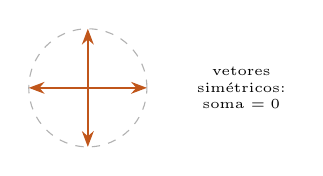
\begin{tikzpicture}[scale=0.75]
        \draw[gray!60, dashed] (0,0) circle (1);
        \foreach \k in {0,1,2,3}
          \draw[->, thick, laranja] (0,0) -- ({90*\k}:1);
        \node[font=\tiny, align=center] at (2.6,0) {vetores\\ simétricos:\\ soma $=0$};
      \end{tikzpicture}
    \end{column}
  \end{columns}
\end{frame}

% =====================================================================
\section{A DFT}
% =====================================================================

\begin{frame}{Transformada discreta de Fourier (DFT)}
  \begin{columns}[T]
    \begin{column}{0.5\textwidth}
      \begin{block}{Definição (DFT)}
        Dado $a = (a_0,\dots,a_{n-1})$, a DFT de $a$ é o vetor
        $y = (y_0,\dots,y_{n-1})$ com
        \[
          y_k = A(\w{k}) = \sum_{j=0}^{n-1} a_j\, \w{kj}.
        \]
        Notação: $y = \DFT_n(a)$.
      \end{block}
      Ou seja: a DFT é a \textbf{avaliação} de $A$ nas $n$ raízes
      $n$-ésimas da unidade.\\[3pt]
      Na multiplicação, o ``$n$'' aqui é o $2n$ da seção anterior.\\[3pt]
      Calcular direto: \alert{$\Theta(n^2)$}.
    \end{column}
    \begin{column}{0.46\textwidth}
      \begin{exampleblock}{Exemplo: $\DFT_4(0,1,2,3)$, \; $\omega_4 = i$}
        \begin{align*}
          y_0 &= 0 + 1 + 2 + 3 = 6\\
          y_1 &= 0 + 1\cdot i + 2\cdot(-1) + 3\cdot(-i)\\
              &= -2 - 2i\\
          y_2 &= 0 + 1\cdot(-1) + 2\cdot 1 + 3\cdot(-1) = -2\\
          y_3 &= 0 + 1\cdot(-i) + 2\cdot(-1) + 3\cdot i\\
              &= -2 + 2i
        \end{align*}
        $y = (6,\; -2-2i,\; -2,\; -2+2i)$.
      \end{exampleblock}
    \end{column}
  \end{columns}
\end{frame}

\begin{frame}{DFT como produto matriz--vetor}
  \begin{columns}[T]
    \begin{column}{0.56\textwidth}
      \small
      A DFT é $y = V_n\,a$, com $V_n$ de Vandermonde nas raízes:
      \[
        \begin{pmatrix} y_0\\ y_1\\ y_2\\ \vdots\\ y_{n-1}\end{pmatrix}
        =
        \begin{pmatrix}
          1 & 1 & 1 & \cdots & 1\\
          1 & \omega_n & \w{2} & \cdots & \w{n-1}\\
          1 & \w{2} & \w{4} & \cdots & \w{2(n-1)}\\
          \vdots & \vdots & \vdots & \ddots & \vdots\\
          1 & \w{n-1} & \w{2(n-1)} & \cdots & \w{(n-1)(n-1)}
        \end{pmatrix}
        \begin{pmatrix} a_0\\ a_1\\ a_2\\ \vdots\\ a_{n-1}\end{pmatrix}
      \]
      Entrada $(k,j)$: $\w{kj}$. Os expoentes formam uma
      \textbf{tabuada} de $0$ a $n-1$.
    \end{column}
    \begin{column}{0.4\textwidth}
      \begin{exampleblock}{Exemplo ($n=4$)}
        \[
          V_4 = \begin{pmatrix}
            1 & 1 & 1 & 1\\
            1 & i & -1 & -i\\
            1 & -1 & 1 & -1\\
            1 & -i & -1 & i
          \end{pmatrix}
        \]
        \[
          V_4 \begin{pmatrix}0\\1\\2\\3\end{pmatrix}
          = \begin{pmatrix}6\\ -2-2i\\ -2\\ -2+2i\end{pmatrix}
        \]
        {\small Ex.: linha 3 tem expoentes $0,3,6,9 \equiv 0,3,2,1 \pmod 4$.}
      \end{exampleblock}
    \end{column}
  \end{columns}
\end{frame}

% =====================================================================
\section{A FFT}
% =====================================================================

\begin{frame}{Divisão e conquista: pares e ímpares}
  \begin{columns}[T]
    \begin{column}{0.52\textwidth}
      Suponha $n$ potência de $2$. Separe os coeficientes de índice par e ímpar
      (limite de grau $n/2$):
      \begin{align*}
        \Aev(x) &= a_0 + a_2x + a_4x^2 + \cdots + a_{n-2}x^{n/2-1}\\
        \Aod(x) &= a_1 + a_3x + a_5x^2 + \cdots + a_{n-1}x^{n/2-1}
      \end{align*}
      \begin{block}{Equação-chave (30.9)}
        \[
          A(x) = \Aev(x^2) + x\,\Aod(x^2)
        \]
      \end{block}
      Avaliar $A$ em $\w{0},\dots,\w{n-1}$ se reduz a:
      \begin{enumerate}
        \item avaliar $\Aev$ e $\Aod$ em $(\w{0})^2,\dots,(\w{n-1})^2$;
        \item combinar pela equação (30.9).
      \end{enumerate}
    \end{column}
    \begin{column}{0.44\textwidth}
      \begin{exampleblock}{Exemplo}
        $A(x) = 0 + 1x + 2x^2 + 3x^3$:
        \begin{align*}
          \Aev(x) &= 0 + 2x\\
          \Aod(x) &= 1 + 3x
        \end{align*}
        Conferindo: $\Aev(x^2) + x\,\Aod(x^2)$\\
        $= 2x^2 + x(1 + 3x^2) = A(x)$.
      \end{exampleblock}
      \begin{alertblock}{Halving em ação}
        \small Os $n$ quadrados $(\w{k})^2$ são só as $n/2$ raízes
        $(n/2)$-ésimas: dois subproblemas $\DFT_{n/2}$ \textbf{do mesmo tipo}.
      \end{alertblock}
    \end{column}
  \end{columns}
\end{frame}

\begin{frame}{O procedimento \proc{FFT}}
  \begin{columns}[T]
    \begin{column}{0.48\textwidth}
      \begin{pseudo}[\small]{\proc{FFT}$(a, n)$}
        \li \IF $n \eqq 1$
        \li[1] \RETURN $a$ \Cm{DFT de 1 elemento}
        \li $\omega_n = e^{2\pi i/n}$
        \li $\omega = 1$
        \li $a^{\mathrm{even}} = (a_0, a_2, \dots, a_{n-2})$
        \li $a^{\mathrm{odd}} = (a_1, a_3, \dots, a_{n-1})$
        \li $\yev = \proc{FFT}(a^{\mathrm{even}}, n/2)$
        \li $\yod = \proc{FFT}(a^{\mathrm{odd}}, n/2)$
        \li \FOR $k = 0$ \TO $n/2 - 1$ \Cm{$\omega = \w{k}$}
        \li[1] $y_k = \yev_k + \omega\,\yod_k$
        \li[1] $y_{k+n/2} = \yev_k - \omega\,\yod_k$
        \li[1] $\omega = \omega\,\omega_n$
        \li \RETURN $y$
      \end{pseudo}
    \end{column}
    \begin{column}{0.48\textwidth}
      \begin{itemize}
        \item \textbf{Linhas 1--2}: caso base, $y_0 = a_0\,\w[1]{0} = a_0$.
        \item \textbf{Linhas 5--8}: dividir e resolver recursivamente:
          \[
            \yev_k = \Aev(\w[n/2]{k}) = \Aev(\w{2k})
          \]
          (lema do cancelamento), e igual para $\yod_k$.
        \item \textbf{Linhas 9--12}: combinar. O valor $\omega$ é atualizado
              iterativamente para não recalcular $\w{k}$.
      \end{itemize}
      \begin{block}{Fatores \textit{twiddle}}
        \small Os $\w{k}$ aparecem com sinal $+$ (linha 10) e $-$ (linha 11):
        são os \textbf{fatores twiddle}.
      \end{block}
    \end{column}
  \end{columns}
\end{frame}

\begin{frame}{Corretude da combinação}
  Para $k = 0,1,\dots,n/2-1$:
  \begin{columns}[T]
    \begin{column}{0.46\textwidth}
      \textbf{Primeira metade} (linha 10):
      \begin{align*}
        y_k &= \yev_k + \w{k}\,\yod_k\\
            &= \Aev(\w{2k}) + \w{k}\,\Aod(\w{2k})\\
            &= A(\w{k}) \quad\text{(por 30.9)}
      \end{align*}
    \end{column}
    \begin{column}{0.5\textwidth}
      \textbf{Segunda metade} (linha 11):
      \begin{align*}
        y_{k+n/2} &= \yev_k - \w{k}\,\yod_k\\
                  &= \yev_k + \w{k+n/2}\,\yod_k \quad (\w{k+n/2} = -\w{k})\\
                  &= \Aev(\w{2k+n}) + \w{k+n/2}\,\Aod(\w{2k+n})\\
                  &= A(\w{k+n/2})
      \end{align*}
      {\small (usando $\w{2k+n} = \w{2k}$.)}
    \end{column}
  \end{columns}
  \vspace{6pt}
  \begin{exampleblock}{Exemplo ($n=4$, $k=1$)}
    $\w[4]{1+2} = \w[4]{3} = -i = -\w[4]{1}$: o mesmo produto $i\cdot\yod_1$ é somado em $y_1$
    e subtraído em $y_3$. Cada multiplicação é aproveitada \textbf{duas vezes}.
  \end{exampleblock}
\end{frame}

\begin{frame}{Exemplo completo: $\proc{FFT}((0,1,2,3), 4)$}
  \begin{columns}[c]
    \begin{column}{0.5\textwidth}
      \centering
      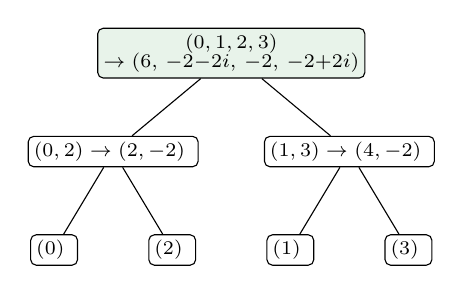
\begin{tikzpicture}[
          level distance=1.25cm,
          level 1/.style={sibling distance=3.0cm},
          level 2/.style={sibling distance=1.5cm},
          every node/.style={tnode}]
        \node[fill=verdeclaro] {$(0,1,2,3)$\\[-1pt] $\to(6,\,-2{-}2i,\,-2,\,-2{+}2i)$}
          child { node {$(0,2)\to(2,-2)$}
            child { node {$(0)$} }
            child { node {$(2)$} } }
          child { node {$(1,3)\to(4,-2)$}
            child { node {$(1)$} }
            child { node {$(3)$} } };
      \end{tikzpicture}

      \vspace{4pt}
      {\scriptsize Cada nó: entrada $\to$ DFT retornada.}
    \end{column}
    \begin{column}{0.46\textwidth}
      \small
      \textbf{Nível $n=2$} ($\omega_2 = -1$, só $k=0$, $\omega=1$):
      \begin{itemize}
        \item $(0,2)$: $y_0 = 0+2 = 2$, \; $y_1 = 0-2 = -2$
        \item $(1,3)$: $y_0 = 1+3 = 4$, \; $y_1 = 1-3 = -2$
      \end{itemize}
      \textbf{Nível $n=4$} ($\omega_4 = i$), $\yev = (2,-2)$, $\yod = (4,-2)$:
      \begin{itemize}
        \item $k=0$, $\omega = 1$:\\
          $y_0 = 2 + 4 = 6$, \; $y_2 = 2 - 4 = -2$
        \item $k=1$, $\omega = i$:\\
          $y_1 = -2 + i(-2) = -2-2i$\\
          $y_3 = -2 - i(-2) = -2+2i$
      \end{itemize}
      Mesmo resultado do cálculo direto da DFT.
    \end{column}
  \end{columns}
\end{frame}

\begin{frame}{Análise da FFT}
  \begin{columns}[T]
    \begin{column}{0.5\textwidth}
      Fora das chamadas recursivas, cada chamada gasta $\Theta(n)$:
      \[
        T(n) = 2T(n/2) + \Theta(n) = \Theta(n\lg n)
      \]
      (caso 2 do teorema mestre).
      \begin{block}{Resultado}
        A FFT avalia um polinômio de limite de grau $n$ nas $n$ raízes $n$-ésimas
        da unidade em $\Theta(n\lg n)$.
      \end{block}
      \begin{alertblock}{Detalhe numérico}
        \small Atualizar $\omega$ iterativamente acumula erros de arredondamento;
        uma alternativa é pré-calcular a tabela dos $\w{k}$.
      \end{alertblock}
    \end{column}
    \begin{column}{0.46\textwidth}
      \centering
      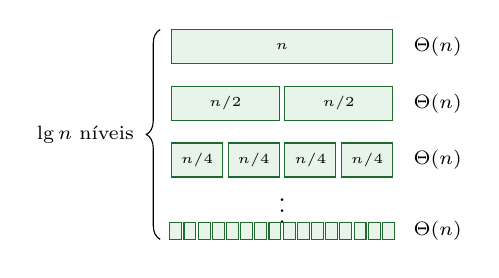
\begin{tikzpicture}[scale=0.72,
          lv/.style={font=\scriptsize, anchor=west}]
        \foreach \y/\m/\c in {0/1/{$n$}, -1/2/{$n/2$}, -2/4/{$n/4$}} {
          \pgfmathsetmacro{\bw}{4.0/\m}
          \foreach \j in {1,...,\m} {
            \draw[fill=verdeclaro, draw=verde] ({(\j-1)*\bw+0.05},\y-0.3) rectangle ({\j*\bw-0.05},\y+0.3);
            \node[font=\tiny] at ({(\j-0.5)*\bw},\y) {\c};
          }
          \node[lv] at (4.15,\y) {$\Theta(n)$};
        }
        \node[font=\small] at (2,-2.75) {$\vdots$};
        \foreach \j in {1,...,16}
          \draw[fill=verdeclaro, draw=verde] ({(\j-1)*0.25+0.02},-3.4) rectangle ({\j*0.25-0.02},-3.1);
        \node[lv] at (4.15,-3.25) {$\Theta(n)$};
        \draw[decorate, decoration={brace, amplitude=5pt, mirror}]
          (-0.15,0.3) -- (-0.15,-3.4) node[midway, left=6pt, font=\scriptsize] {$\lg n$ níveis};
      \end{tikzpicture}\\[4pt]
      {\small $\lg n$ níveis $\times$ $\Theta(n)$ por nível.}\\[4pt]
      {\small Ex.: $n = 1024$: DFT direta $\approx 10^6$ operações; FFT $\approx 10^4$.}
    \end{column}
  \end{columns}
\end{frame}

% =====================================================================
\section{Interpolação e DFT inversa}
% =====================================================================

\begin{frame}{A inversa de $V_n$}
  \begin{columns}[T]
    \begin{column}{0.52\textwidth}
      Para interpolar, precisamos de $a = V_n^{-1} y$.
      \begin{block}{Teorema 30.7}
        Para $j,k = 0,\dots,n-1$, a entrada $(j,k)$ de $V_n^{-1}$ é
        \[
          \big[V_n^{-1}\big]_{jk} = \w{-jk}/n.
        \]
      \end{block}
      \textbf{Prova}: entrada $(k,k')$ de $V_n^{-1}V_n$:
      \[
        \sum_{j=0}^{n-1} \frac{\w{-jk}}{n}\,\w{jk'} = \frac{1}{n}\sum_{j=0}^{n-1}\w{j(k'-k)}
      \]
      $= 1$ se $k'=k$; e $= 0$ caso contrário, pelo \textbf{lema do somatório}
      ($-(n-1) \le k'-k \le n-1$, logo $n \nmid k'-k$).
    \end{column}
    \begin{column}{0.44\textwidth}
      \small
      \begin{exampleblock}{Exemplo ($n=2$, $\omega_2 = -1$)}
        \[
          V_2 = \begin{pmatrix} 1 & 1\\ 1 & -1\end{pmatrix},\quad
          V_2^{-1} = \frac12\begin{pmatrix} 1 & 1\\ 1 & -1\end{pmatrix}
        \]
        Conferindo: $V_2^{-1}V_2 = \frac12\begin{pmatrix} 2 & 0\\ 0 & 2\end{pmatrix} = I$
      \end{exampleblock}
      \begin{exampleblock}{Exemplo ($n=4$, $\w[4]{-1} = -i$)}
        \[
          V_4^{-1} = \frac14\begin{pmatrix}
            1 & 1 & 1 & 1\\
            1 & -i & -1 & i\\
            1 & -1 & 1 & -1\\
            1 & i & -1 & -i
          \end{pmatrix}
        \]
      \end{exampleblock}
    \end{column}
  \end{columns}
\end{frame}

\begin{frame}{DFT inversa com a FFT}
  \begin{columns}[T]
    \begin{column}{0.5\textwidth}
      \vspace{-6pt}
      \begin{align*}
        \text{DFT inversa:}\quad a_j &= \frac{1}{n}\sum_{k=0}^{n-1} y_k\, \w{-kj}\\
        \text{DFT:}\quad y_k &= \sum_{j=0}^{n-1} a_j\,\w{kj}
      \end{align*}
      Basta modificar a \proc{FFT}:
      \begin{enumerate}
        \item trocar os papéis de $a$ e $y$;
        \item usar $\omega_n^{-1} = e^{-2\pi i/n}$ no lugar de $\omega_n$ (linha 3);
        \item dividir cada elemento do resultado por $n$.
      \end{enumerate}
      $\Rightarrow$ $\DFT_n^{-1}$ também em \textbf{$\Theta(n\lg n)$}.
    \end{column}
    \begin{column}{0.46\textwidth}
      \begin{exampleblock}{Exemplo: $\DFT_4^{-1}(6,\,-2{-}2i,\,-2,\,-2{+}2i)$}
        Potências de $\w[4]{-1} = -i$ para $j=1$: $1,\,-i,\,-1,\,i$.
        \begin{align*}
          a_1 &= \tfrac14\big[6 + (-2{-}2i)(-i) + (-2)(-1)\\
              &\qquad + (-2{+}2i)(i)\big]\\
              &= \tfrac14\big[6 + (-2{+}2i) + 2 + (-2{-}2i)\big]\\
              &= \tfrac44 = 1
        \end{align*}
        Da mesma forma, $a_0 = \tfrac14(6 - 2 - 2 - 2) = 0$, $a_2 = 2$ e $a_3 = 3$.\\
        Recuperamos $a = (0,1,2,3)$.
      \end{exampleblock}
    \end{column}
  \end{columns}
\end{frame}

\begin{frame}{Teorema da convolução}
  \begin{block}{Teorema 30.8 (convolução)}
    Para vetores $a$ e $b$ de comprimento $n$ (potência de 2), completados com zeros até $2n$:
    \[
      a \otimes b = \DFT_{2n}^{-1}\big(\DFT_{2n}(a) \cdot \DFT_{2n}(b)\big),
    \]
    onde $\cdot$ é o produto componente a componente.
  \end{block}
  \vspace{4pt}
  \centering
  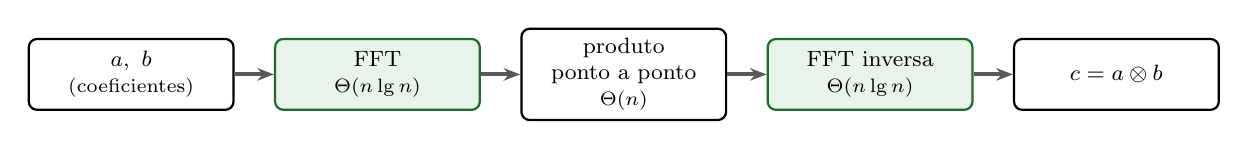
\begin{tikzpicture}[node distance=0.5cm]
    \node[bloco] (a) {$a,\ b$\\ \scriptsize (coeficientes)};
    \node[destaque, right=of a] (f) {FFT\\ \scriptsize $\Theta(n\lg n)$};
    \node[bloco, right=of f] (m) {produto\\ ponto a ponto\\ \scriptsize $\Theta(n)$};
    \node[destaque, right=of m] (fi) {FFT inversa\\ \scriptsize $\Theta(n\lg n)$};
    \node[bloco, right=of fi] (c) {$c = a\otimes b$};
    \draw[seta] (a) -- (f);
    \draw[seta] (f) -- (m);
    \draw[seta] (m) -- (fi);
    \draw[seta] (fi) -- (c);
  \end{tikzpicture}

  \vspace{8pt}
  \raggedright
  {\small Multiplicar polinômios $\equiv$ convoluir seus vetores de coeficientes
  $\equiv$ multiplicar ponto a ponto no ``domínio da frequência''.}
\end{frame}

\begin{frame}{Exemplo: $(1+2x)(3+x)$ com a FFT}
  \begin{columns}[T]
    \begin{column}{0.5\textwidth}
      \small
      \textbf{1. Completar com zeros} ($2n = 4$, $\omega_4 = i$):\\
      $a = (1,2,0,0)$, \; $b = (3,1,0,0)$

      \vspace{4pt}
      \textbf{2. Avaliar} ($y_k = A(i^k)$):
      \begin{center}
        \begin{tabular}{ccccc}
          \toprule
          $k$ & $0$ & $1$ & $2$ & $3$ \\
          $x = i^k$ & $1$ & $i$ & $-1$ & $-i$ \\
          \midrule
          $A = 1{+}2x$ & $3$ & $1{+}2i$ & $-1$ & $1{-}2i$ \\
          $B = 3{+}x$  & $4$ & $3{+}i$ & $2$ & $3{-}i$ \\
          \midrule
          $C = A\cdot B$ & $12$ & $1{+}7i$ & $-2$ & $1{-}7i$ \\
          \bottomrule
        \end{tabular}
      \end{center}
      {\scriptsize $(1{+}2i)(3{+}i) = 3 + i + 6i + 2i^2 = 1 + 7i$.}
    \end{column}
    \begin{column}{0.46\textwidth}
      \small
      \textbf{3. Interpolar} ($c_j = \frac14\sum_k C_k (-i)^{kj}$):
      \begin{align*}
        c_0 &= \tfrac14(12 + 1{+}7i - 2 + 1{-}7i) = 3\\
        c_1 &= \tfrac14(12 + (7{-}i) + 2 + (7{+}i)) = 7\\
        c_2 &= \tfrac14(12 - (1{+}7i) - 2 - (1{-}7i)) = 2\\
        c_3 &= \tfrac14(12 + (i{-}7) + 2 + (-7{-}i)) = 0
      \end{align*}
      \begin{exampleblock}{Resultado}
        $C(x) = 3 + 7x + 2x^2$ --- igual à convolução direta feita na Introdução.
      \end{exampleblock}
    \end{column}
  \end{columns}
\end{frame}

% =====================================================================
\section{Circuitos da FFT}
% =====================================================================

\begin{frame}{Operação \textit{butterfly}}
  \begin{columns}[c]
    \begin{column}{0.48\textwidth}
      As linhas 10--11 da \proc{FFT} calculam $\w{k}\yod_k$ duas vezes. Com uma
      variável temporária:
      \begin{pseudo}[\small]{}
        \li $t = \omega\, \yod_k$
        \li $y_k = \yev_k + t$
        \li $y_{k+n/2} = \yev_k - t$
      \end{pseudo}
      \vspace{4pt}
      Multiplicar pelo fator twiddle, somar e subtrair: operação
      \textbf{borboleta} (\textit{butterfly}).
      \begin{exampleblock}{Exemplo}
        $\yev_1 = -2$, $\yod_1 = -2$, $\omega = \w[4]{1} = i$:\\
        $t = -2i$; \; $y_1 = -2-2i$; \; $y_3 = -2+2i$.
      \end{exampleblock}
    \end{column}
    \begin{column}{0.48\textwidth}
      \centering
      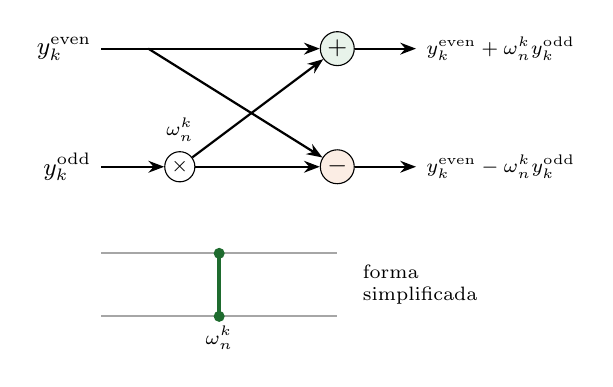
\begin{tikzpicture}[scale=1.0]
        \node[font=\small, anchor=east] (e) at (0,1.5) {$\yev_k$};
        \node[font=\small, anchor=east] (o) at (0,0) {$\yod_k$};
        \node[draw, circle, inner sep=1pt, font=\scriptsize, fill=white] (mul) at (1,0) {$\times$};
        \node[font=\scriptsize, above] at (mul.north) {$\w{k}$};
        \node[draw, circle, inner sep=1pt, font=\small, fill=verdeclaro] (p) at (3,1.5) {$+$};
        \node[draw, circle, inner sep=1pt, font=\small, fill=laranjaclaro] (m) at (3,0) {$-$};
        \draw[->, thick] (e.east) -- (p);
        \draw[->, thick] (o.east) -- (mul);
        \draw[->, thick] (mul) -- (m);
        \draw[->, thick] (0.6,1.5) -- (m);
        \draw[->, thick] (mul) -- (p);
        \draw[->, thick] (p) -- (4,1.5) node[right, font=\scriptsize] {$\yev_k + \w{k}\yod_k$};
        \draw[->, thick] (m) -- (4,0) node[right, font=\scriptsize] {$\yev_k - \w{k}\yod_k$};
        % versão simplificada
        \begin{scope}[yshift=-1.9cm]
          \draw[fio] (0,0.8) -- (3,0.8);
          \draw[fio] (0,0) -- (3,0);
          \draw[bf] (1.5,0.8) -- (1.5,0);
          \node[bfdot] at (1.5,0.8) {};
          \node[bfdot] at (1.5,0) {};
          \node[font=\scriptsize, below] at (1.5,0) {$\w{k}$};
          \node[font=\scriptsize, anchor=west, align=left] at (3.2,0.4) {forma\\ simplificada};
        \end{scope}
      \end{tikzpicture}
    \end{column}
  \end{columns}
\end{frame}

\begin{frame}{Permutação por inversão de bits}
  \begin{columns}[c]
    \begin{column}{0.54\textwidth}
      \centering
      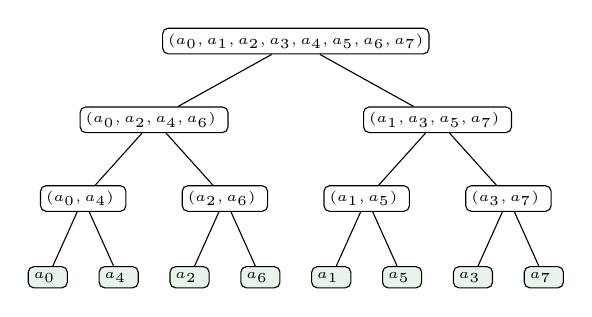
\begin{tikzpicture}[
          level distance=1.0cm,
          level 1/.style={sibling distance=3.6cm},
          level 2/.style={sibling distance=1.8cm},
          level 3/.style={sibling distance=0.9cm},
          every node/.style={tnode, font=\tiny}]
        \node {$(a_0,a_1,a_2,a_3,a_4,a_5,a_6,a_7)$}
          child { node {$(a_0,a_2,a_4,a_6)$}
            child { node {$(a_0,a_4)$}
              child { node[fill=verdeclaro] {$a_0$} } child { node[fill=verdeclaro] {$a_4$} } }
            child { node {$(a_2,a_6)$}
              child { node[fill=verdeclaro] {$a_2$} } child { node[fill=verdeclaro] {$a_6$} } } }
          child { node {$(a_1,a_3,a_5,a_7)$}
            child { node {$(a_1,a_5)$}
              child { node[fill=verdeclaro] {$a_1$} } child { node[fill=verdeclaro] {$a_5$} } }
            child { node {$(a_3,a_7)$}
              child { node[fill=verdeclaro] {$a_3$} } child { node[fill=verdeclaro] {$a_7$} } } };
      \end{tikzpicture}\\[2pt]
      {\scriptsize Árvore de chamadas recursivas da \proc{FFT} para $n=8$.}
    \end{column}
    \begin{column}{0.42\textwidth}
      As folhas aparecem na ordem $0,4,2,6,1,5,3,7$: o elemento $a_k$ vai para a posição
      $\mathrm{rev}(k)$ (bits de $k$ invertidos).
      \begin{exampleblock}{Exemplo ($\lg n = 3$ bits)}
        \centering\small
        \begin{tabular}{cccc}
          \toprule
          $k$ & binário & invertido & $\mathrm{rev}(k)$ \\
          \midrule
          $1$ & $001$ & $100$ & $4$ \\
          $3$ & $011$ & $110$ & $6$ \\
          $6$ & $110$ & $011$ & $3$ \\
          \bottomrule
        \end{tabular}
      \end{exampleblock}
      {\small Motivo: em cada nível, o bit menos significativo decide se o índice vai
      para a esquerda (par) ou direita (ímpar).}
    \end{column}
  \end{columns}
\end{frame}

\begin{frame}{O circuito completo da FFT ($n=8$)}
  \begin{columns}[c]
    \begin{column}{0.58\textwidth}
      \centering
      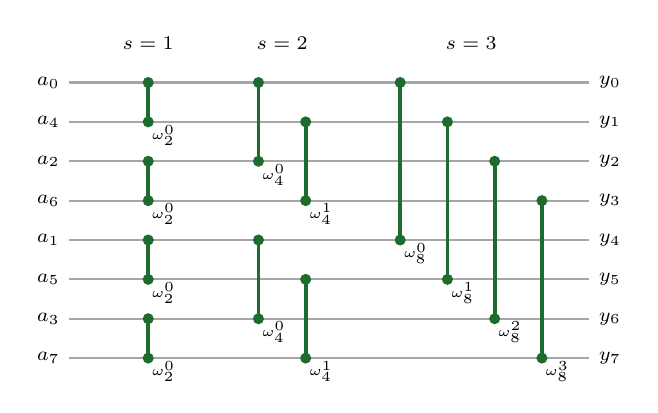
\begin{tikzpicture}[yscale=-0.5, xscale=1.0]
        % fios
        \foreach \p/\a in {0/0,1/4,2/2,3/6,4/1,5/5,6/3,7/7} {
          \draw[fio] (0,\p) -- (6.6,\p);
          \node[font=\scriptsize, anchor=east] at (0,\p) {$a_{\a}$};
          \node[font=\scriptsize, anchor=west] at (6.6,\p) {$y_{\p}$};
        }
        % estágio 1: pares (0,1),(2,3),(4,5),(6,7), twiddle w_2^0
        \foreach \t in {0,2,4,6} {
          \draw[bf] (1.0,\t) -- (1.0,\t+1);
          \node[bfdot] at (1.0,\t) {}; \node[bfdot] at (1.0,\t+1) {};
          \node[font=\tiny, anchor=north west, inner sep=1pt] at (1.0,\t+1) {$\w[2]{0}$};
        }
        % estágio 2: grupos de 4
        \foreach \g in {0,4} {
          \foreach \j in {0,1} {
            \pgfmathsetmacro{\x}{2.4+0.6*\j}
            \draw[bf] (\x,\g+\j) -- (\x,\g+\j+2);
            \node[bfdot] at (\x,\g+\j) {}; \node[bfdot] at (\x,\g+\j+2) {};
            \node[font=\tiny, anchor=north west, inner sep=1pt] at (\x,\g+\j+2) {$\w[4]{\j}$};
          }
        }
        % estágio 3: um grupo de 8
        \foreach \j in {0,1,2,3} {
          \pgfmathsetmacro{\x}{4.2+0.6*\j}
          \draw[bf] (\x,\j) -- (\x,\j+4);
          \node[bfdot] at (\x,\j) {}; \node[bfdot] at (\x,\j+4) {};
          \node[font=\tiny, anchor=north west, inner sep=1pt] at (\x,\j+4) {$\w[8]{\j}$};
        }
        \node[font=\scriptsize] at (1.0,-1) {$s=1$};
        \node[font=\scriptsize] at (2.7,-1) {$s=2$};
        \node[font=\scriptsize] at (5.1,-1) {$s=3$};
      \end{tikzpicture}
    \end{column}
    \begin{column}{0.38\textwidth}
      \small
      \begin{itemize}
        \item Entradas em ordem de \textbf{inversão de bits}.
        \item $\lg n$ estágios; cada um com $n/2$ borboletas \textbf{em paralelo}.
        \item Estágio $s$: $n/2^s$ grupos com $2^{s-1}$ borboletas; twiddles
              $\w[m]{0},\dots,\w[m]{m/2-1}$, $m = 2^s$.
      \end{itemize}
      \begin{block}{Custo}
        Profundidade $\Theta(\lg n)$;\\
        $\Theta(n\lg n)$ borboletas no total.
      \end{block}
    \end{column}
  \end{columns}
\end{frame}

\begin{frame}{Exemplo: circuito para $a = (0,1,2,3)$}
  \begin{columns}[c]
    \begin{column}{0.56\textwidth}
      \centering
      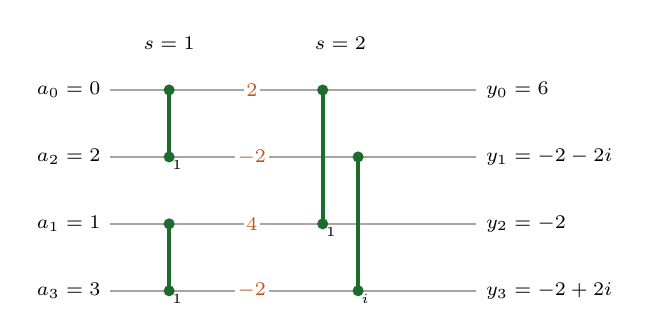
\begin{tikzpicture}[yscale=-0.85, xscale=0.75]
        \foreach \p/\a in {0/0,1/2,2/1,3/3}
          \draw[fio] (0,\p) -- (6.2,\p);
        % entradas (ordem invertida: a0,a2,a1,a3)
        \foreach \p/\lab in {0/{$a_0=0$},1/{$a_2=2$},2/{$a_1=1$},3/{$a_3=3$}}
          \node[font=\scriptsize, anchor=east] at (0,\p) {\lab};
        % estágio 1
        \foreach \t in {0,2} {
          \draw[bf] (1.0,\t) -- (1.0,\t+1);
          \node[bfdot] at (1.0,\t) {}; \node[bfdot] at (1.0,\t+1) {};
          \node[font=\tiny, anchor=north west, inner sep=1pt] at (1.0,\t+1) {$1$};
        }
        % valores intermediários
        \foreach \p/\v in {0/2,1/{-2},2/4,3/{-2}}
          \node[font=\scriptsize, fill=white, inner sep=1pt, text=laranja] at (2.4,\p) {$\v$};
        % estágio 2
        \foreach \j/\tw in {0/1,1/i} {
          \pgfmathsetmacro{\x}{3.6+0.6*\j}
          \draw[bf] (\x,\j) -- (\x,\j+2);
          \node[bfdot] at (\x,\j) {}; \node[bfdot] at (\x,\j+2) {};
          \node[font=\tiny, anchor=north west, inner sep=1pt] at (\x,\j+2) {$\tw$};
        }
        \foreach \p/\v in {0/{y_0=6},1/{y_1=-2-2i},2/{y_2=-2},3/{y_3=-2+2i}}
          \node[font=\scriptsize, anchor=west] at (6.2,\p) {$\v$};
        \node[font=\scriptsize] at (1.0,-0.7) {$s=1$};
        \node[font=\scriptsize] at (3.9,-0.7) {$s=2$};
      \end{tikzpicture}
    \end{column}
    \begin{column}{0.4\textwidth}
      \small
      \textbf{Estágio 1} (twiddle $\w[2]{0}=1$):
      \begin{itemize}
        \item $(0,2) \to (0+2,\ 0-2) = (2,-2)$
        \item $(1,3) \to (1+3,\ 1-3) = (4,-2)$
      \end{itemize}
      \textbf{Estágio 2} (twiddles $\w[4]{0}=1$, $\w[4]{1}=i$):
      \begin{itemize}
        \item fios 0 e 2: $2 \pm 1\cdot 4 = 6,\ -2$
        \item fios 1 e 3: $-2 \pm i\cdot(-2) = -2-2i,\ -2+2i$
      \end{itemize}
      O circuito executa a recursão \textbf{de baixo para cima} e chega à mesma DFT.
    \end{column}
  \end{columns}
\end{frame}

% =====================================================================
\section{Fechamento}
% =====================================================================

\begin{frame}{Fechamento}
  \begin{columns}[T]
    \begin{column}{0.44\textwidth}
      \small
      \textbf{Como as peças se encaixam:}
      \begin{itemize}
        \item \textbf{Cancelamento} $\Rightarrow$ \textbf{halving}: os quadrados das raízes
              são metade delas $\Rightarrow$ subproblemas de tamanho $n/2$.
        \item $\w{k+n/2} = -\w{k}$ $\Rightarrow$ cada produto serve para duas saídas (\textit{butterfly}).
        \item \textbf{Somatório} $\Rightarrow$ $V_n^{-1}$ tem forma simples $\Rightarrow$
              a mesma FFT faz a interpolação.
        \item Estrutura recursiva $\Rightarrow$ circuito paralelo de profundidade $\Theta(\lg n)$.
      \end{itemize}
    \end{column}
    \begin{column}{0.54\textwidth}
      \centering\footnotesize
      \begin{tabular}{@{}lcc@{}}
        \toprule
        Operação & Coeficientes & Pontos \\
        \midrule
        Avaliar em 1 ponto  & $\Theta(n)$ & --- \\
        Soma                & $\Theta(n)$ & $\Theta(n)$ \\
        Multiplicação       & $\Theta(n^2)$ & $\Theta(n)$ \\
        \midrule
        \multicolumn{3}{@{}l}{\textit{Conversões}} \\
        Avaliar em $n$ pontos & \multicolumn{2}{c}{$\Theta(n^2)$} \\
        Interpolar (Lagrange) & \multicolumn{2}{c}{$\Theta(n^2)$} \\
        DFT / DFT$^{-1}$ via FFT & \multicolumn{2}{c}{$\Theta(n\lg n)$} \\
        \midrule
        \textbf{Multiplicação via FFT} & \multicolumn{2}{c}{$\bm{\Theta(n\lg n)}$} \\
        \bottomrule
      \end{tabular}
    \end{column}
  \end{columns}
\end{frame}

\begin{frame}[standout]
  Obrigado!
\end{frame}

\end{document}
